\documentclass{article}

\usepackage{arxiv}

\usepackage[utf8]{inputenc} % allow utf-8 input
\usepackage[T1]{fontenc}    % use 8-bit T1 fonts
\usepackage{hyperref}       % hyperlinks
\usepackage{url}            % simple URL typesetting
\usepackage{booktabs}       % professional-quality tables
\usepackage{amsfonts}       % blackboard math symbols
\usepackage{nicefrac}       % compact symbols for 1/2, etc.
\usepackage{microtype}      % microtypography
\usepackage{cleveref}       % smart cross-referencing
\usepackage{lipsum}         % Can be removed after putting your text content
\usepackage{tabularx} % Add this to your preamble
\usepackage{placeins}
\usepackage{graphicx}
\usepackage{natbib}
\usepackage{doi}

\raggedbottom % Allow uneven spacing


\title{Thread and Process Management in QNX Neutrino RTOS}

% Here you can change the date presented in the paper title
%\date{September 9, 1985}
% Or remove it
%\date{}

\newif\ifuniqueAffiliation
% Comment to use multiple affiliations variant of author block 
\uniqueAffiliationtrue

\ifuniqueAffiliation % Standard variant of author block
\author{ 
	\href{https://orcid.org/0009-0000-3709-0802}{
\includegraphics[scale=0.06]{orcid.pdf}\hspace{1mm}Jakub Oleszczuk} \\
	Faculty of Transport, Electrical Engineering and Computer Science\\
	University of Radom\\
	Radom, Poland \\
	\texttt{118060@student.uthrad.pl} \\
}
\else
% Multiple affiliations variant of author block
\usepackage{authblk}
\renewcommand\Authfont{\bfseries}
\setlength{\affilsep}{0em}
% box is needed for correct spacing with authblk
\newbox{\orcid}\sbox{\orcid}{
\includegraphics[scale=0.06]{orcid.pdf}} 
\author[1]{%
	\href{https://orcid.org/0009-0000-3709-0802}{\usebox{\orcid}\hspace{1mm}Jakub Oleszczuk\thanks{\texttt{118060@student.uthrad.pl}}}%
}
\affil[1]{Faculty of Transport, Electrical Engineering and Computer Science, University of Radom, Radom,26-600, Poland}
\fi

% Uncomment to override  the `A preprint' in the header
\renewcommand{\headeright}{Technical Report}
\renewcommand{\undertitle}{Technical Report}
\renewcommand{\shorttitle}{Thread and Process Management in QNX Neutrino RTOS}

%%% Add PDF metadata to help others organize their library
%%% Once the PDF is generated, you can check the metadata with
%%% $ pdfinfo template.pdf
\hypersetup{
pdftitle={Thread and Process Management in QNX Neutrino RTOS},
pdfsubject={q-bio.NC, q-bio.QM},
pdfauthor={Jakub Oleszczuk},
pdfkeywords={QNX Neutrino, RTOS, Thread Management, Process Management},
}

\begin{document}
\maketitle

\begin{abstract}
	\label{sec:abstract}

	This paper presents the thread and process management mechanism of the QNX Neutrino real-time operating system.
	The aim is to highlight how QNX, as microkernel-based RTOS, handles concurrency and determinism in time-critical applications.
	The paper discusses the internal structure of threads and processes, their interaction, and real-time scheduling policies such as $SCHED\_FIFO$
	and sporadic context of avoiding priority inversion and ensuring system reliability. The presented features make QNX Neutrino suitable for
	embedded and mission-critical systems.

\end{abstract}


% keywords can be removed
\keywords{QNX Neutrino \and RTOS \and Thread Management \and Process Management}


\section{Introduction}
\label{sec:intro}
RTOSs are designed to serve real-time applications that process data as it comes in, typically without any buffering delays.
The QNX Neutrino RTOS \citep{WhatsRTOS2024} is a microkernel-based operating system that provides a high degree of concurrency and real-time performance.
It is widely used in embedded systems, automotive applications, and other mission-critical environments.
The QNX Neutrino RTOS is designed to be modular and scalable, allowing developers to customize the system to meet the specific needs of their applications.

\subsection{RTOS vs General-Purpose OS}
\label{sec:rtos-vs-gpos}
Real-time operating systems (RTOS) are designed to meet the timing constraints of real-time applications, while general-purpose operating systems (GPOS) are designed for a wide range of applications and do not have the same timing constraints.
RTOSs are typically used in embedded systems, automotive applications, and other mission-critical environments where timing is critical.
GPOSs are typically used in desktop and server environments where timing is not as critical.

\begin{table}[!ht]
    \centering
    \small % Reduce font size
    \begin{tabularx}{\textwidth}{@{}Xl@{}}
        \toprule
        Advantages  & Disadvantages   \\ \midrule
        Fault isolation and recovery for high availability. & Requires more context switching, which can increase overhead. \\ \hline
        Restart a failed system service dynamically without impacts to the kernel (no system reboot). & \\ \hline
        Easy expansion—develop device drivers and OS extensions without a kernel guru and without recompiling. & \\ \hline
        Easier to debug. & \\ \hline
        Small footprint. & \\ \hline
        Less code running in kernel space reduces attack surface and increases security. & \\ \bottomrule
    \end{tabularx}
    \caption{Advantages and Disadvantages of a Microkernel RTOS (e.g. QNX Neutrino RTOS) \citep{WhatsRTOS2024}}
    \label{tab:microkernel-advantages}
\end{table}

\subsection{QNX SDP 8.0}
\label{sec:qnx-sdp}
The QNX Software Development Platform (SDP) 8.0 is the latest version of the QNX Neutrino RTOS, which provides a comprehensive development environment for building real-time applications.
The SDP 8.0 includes a wide range of tools and libraries for developing, debugging, and deploying applications on QNX Neutrino.
The SDP 8.0 includes a new set of development tools, including the QNX Momentics IDE, which provides a powerful and flexible environment for developing real-time applications.


\subsection{QNX Neutrino}
\label{sec:qnx-neutrino}
Although QNX SDP 7.0 was the classical distribution focused exclusively on Neutrino RTOS, the more recent SDP 8.0 (released in 2023) introduces enhanced development tools,
still incorporates Neutrino's real-time capabilities with improved development tooling and broader system integration.
The QNX Neutrino RTOS is a microkernel-based operating system that provides a high degree of concurrency and real-time performance.
It is widely used in embedded systems, automotive applications, and other mission-critical environments.

\subsection{QNX Momentics}
\label{sec:qnx-momentics}
The QNX Momentics IDE is a powerful development environment that provides a wide range of tools for developing, debugging, and deploying applications on QNX Neutrino.
The IDE includes a code editor, a debugger, and a profiler, as well as tools for managing projects and building applications.
The QNX Momentics IDE is designed to be easy to use and provides a wide range of features for developing real-time applications.
 
\begin{figure}[!htbp]
    \centering
    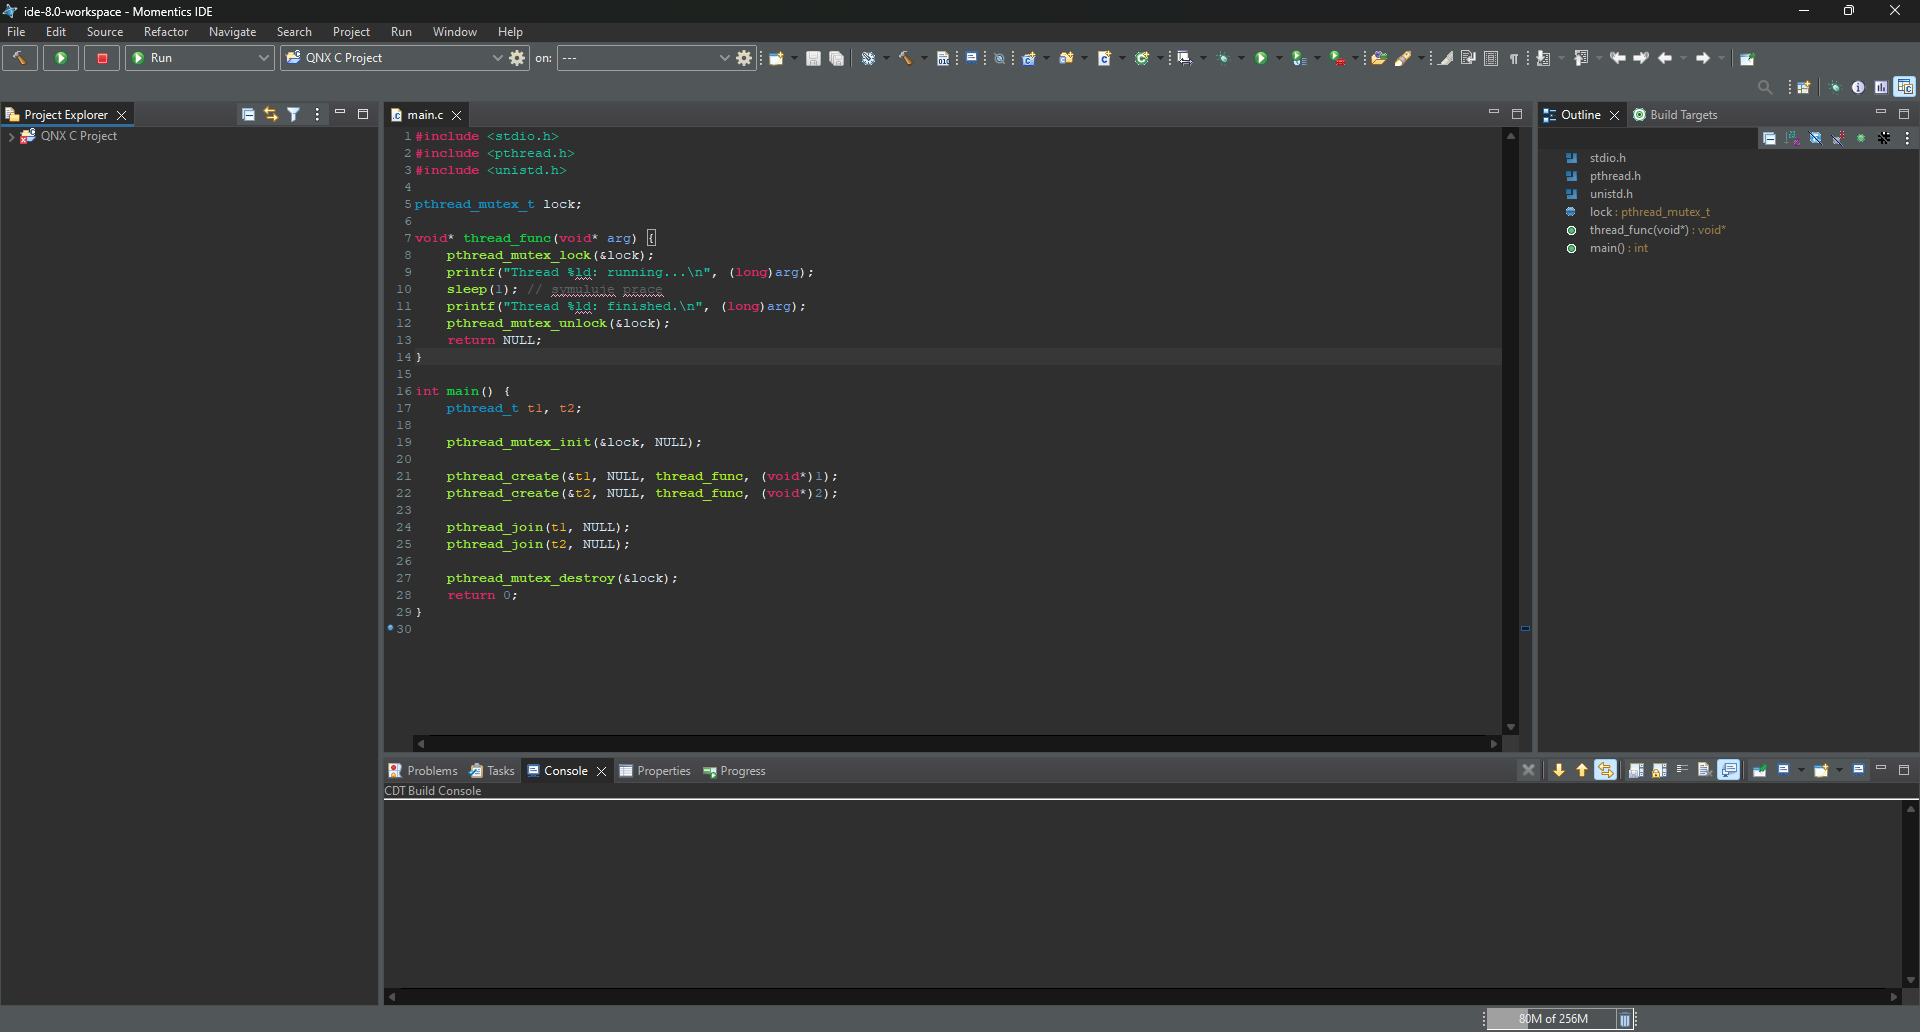
\includegraphics[width=0.8\textwidth]{graph2.png} % Replace 'image.png' with your image file name
    \caption{QNX Momentics IDE Window \citep{qnx_m} }
    \label{fig:qnx-momentics window}
\end{figure}

\section{Monolithic vs Microkernel Architecture}
\label{sec:monolithic-vs-microkernel}

For operating systems, the architecture can be broadly classified into two categories: monolithic and microkernel.
Monolithic operating systems have a single large kernel that manages all system resources and services, while microkernel operating systems have a small kernel that provides only the most essential services, with other services running in user space.
Monolithic kernels are typically larger and more complex than microkernels, as they include all the necessary services and drivers within the kernel itself.
This can make monolithic kernels more difficult to maintain and debug, as any changes to the kernel can affect the entire system.
Microkernels, on the other hand, are designed to be modular and extensible, allowing developers to add or remove services as needed.
This modularity can make microkernels easier to maintain and debug, as changes to one service do not affect the entire system.
Monolithic kernels are typically faster than microkernels, as they do not require the overhead of inter-process communication (IPC) between user space and kernel space.
However, microkernels can provide better fault isolation and recovery, as services running in user space can be restarted or replaced without affecting the kernel or other services.
Monolithic kernels are typically used in general-purpose operating systems, such as Linux and Windows, while microkernels are used in real-time operating systems (RTOS), such as QNX Neutrino and VxWorks.
The microkernel architecture is designed to be modular and extensible, allowing developers to add or remove services as needed.

\begin{figure}[h!]
    \centering
    \begin{minipage}{0.45\textwidth}
        \centering
        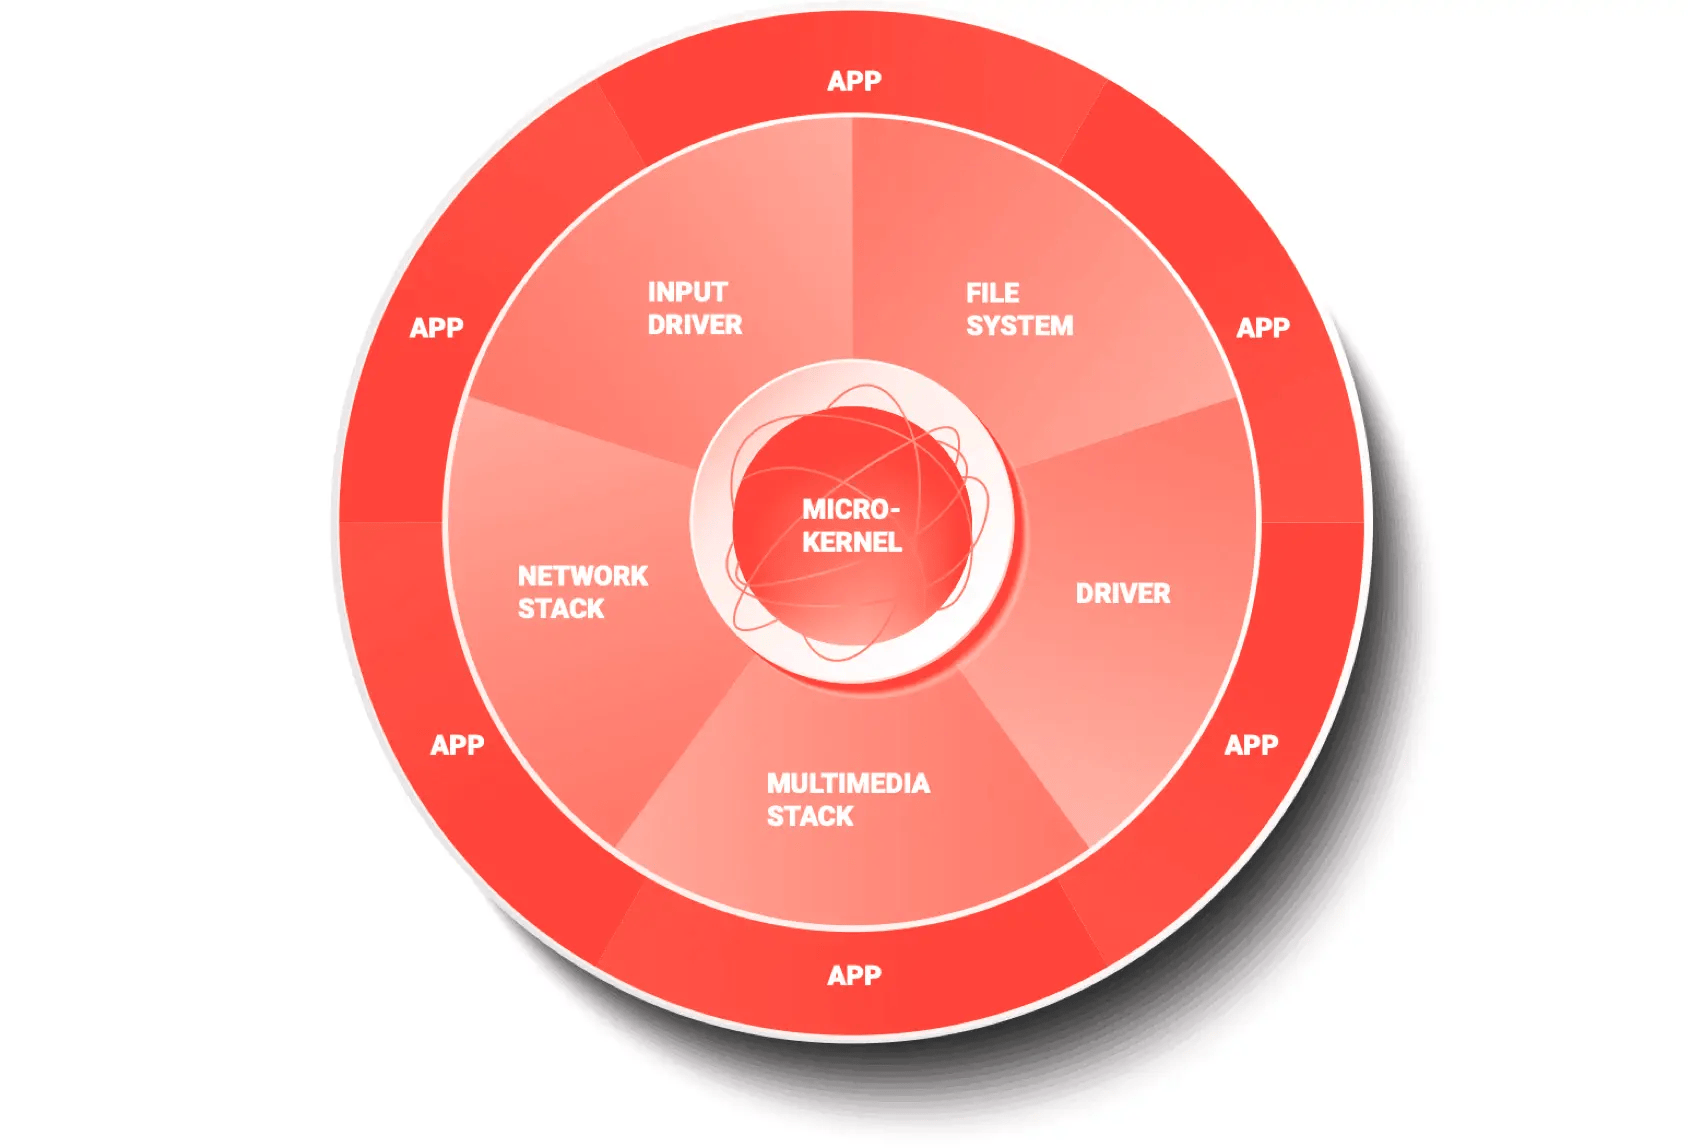
\includegraphics[width=\textwidth]{graph1.png} % Replace with your image file
        \caption{Microkernel OS architecture diagram \citep{WhatsRTOS2024}}
        \label{fig:microkernel}
    \end{minipage}
    \hfill
    \begin{minipage}{0.45\textwidth}
        \centering
        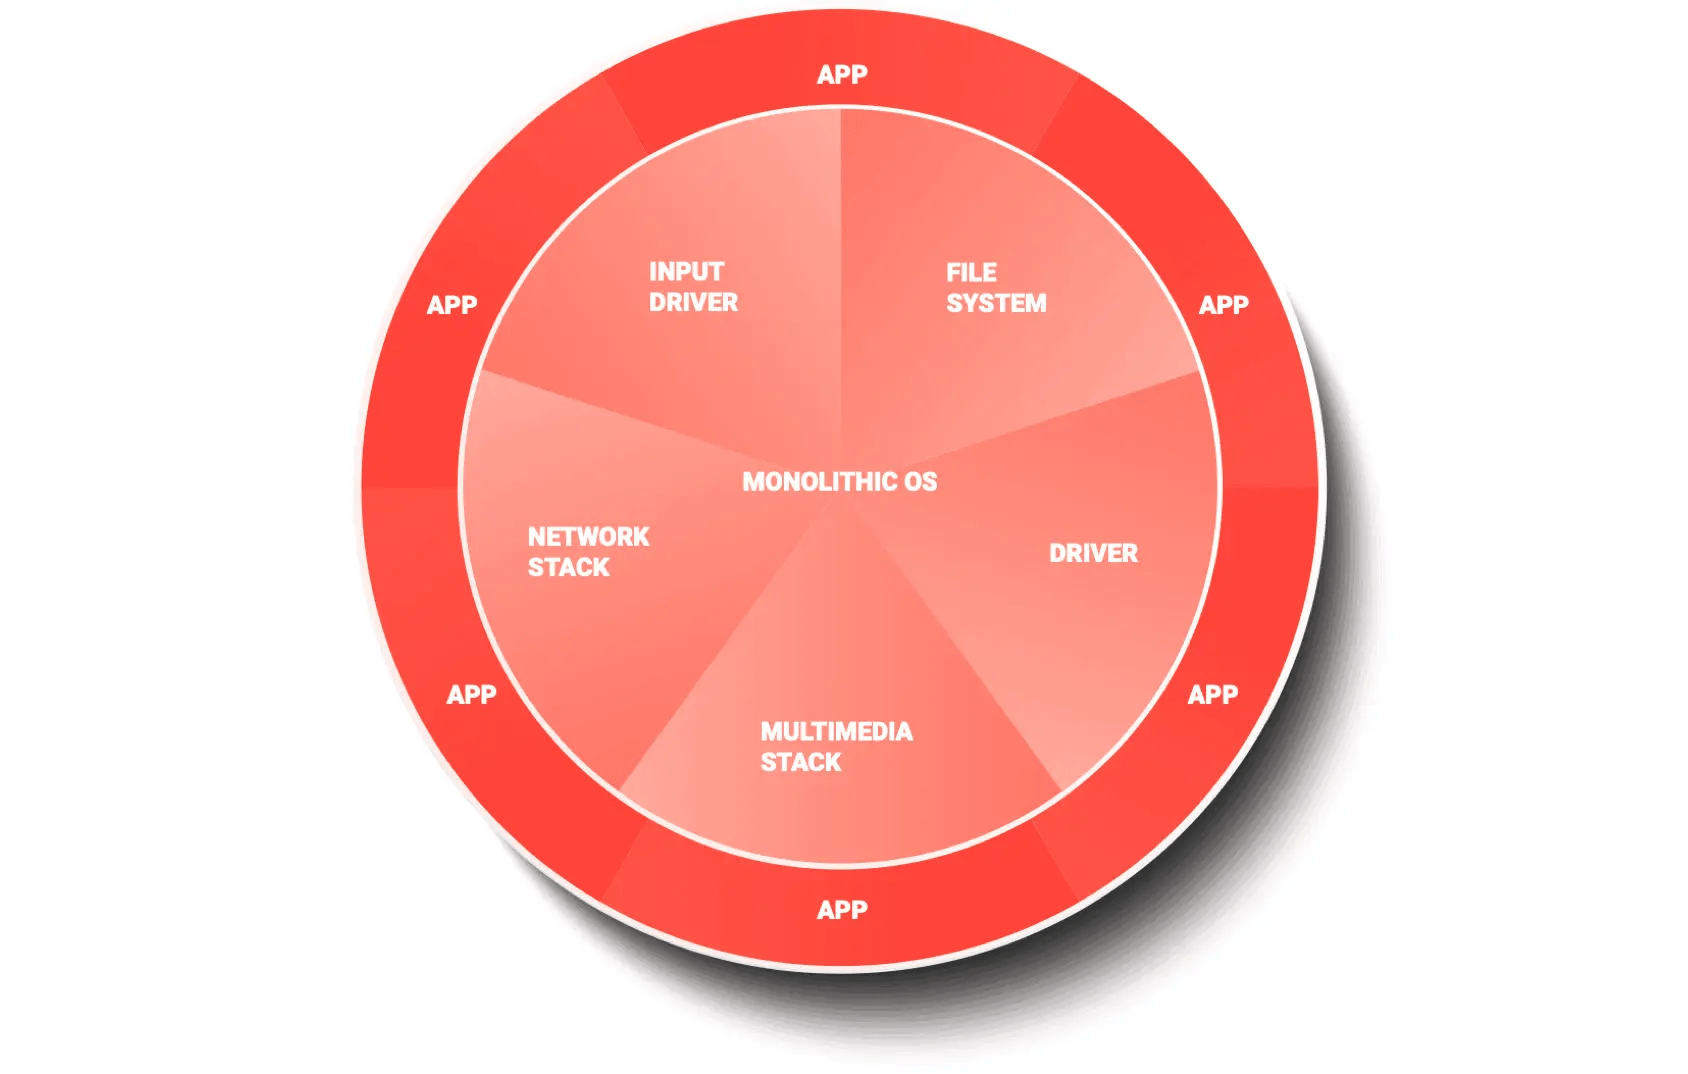
\includegraphics[width=\textwidth]{graph3.png} % Replace with your image file
        \caption{Monolithic OS architecture diagram \citep{WhatsRTOS2024}}
        \label{fig:monolithic}
    \end{minipage}
\end{figure}
\FloatBarrier

\section{POSIX Standard}
\label{sec:posix-standard}
The Portable Operating System Interface (POSIX) is a set of standards that define the application programming interface (API), along with command line shells and utility interfaces, for software compatibility with variants of Unix and other operating systems.
The POSIX standard is designed to provide a consistent and portable interface for developing applications that can run on different operating systems.
The POSIX standard provides a set of APIs and standards for developing portable applications that can run on different operating systems.

\subsection{QNX Neutrino RTOS and POSIX}
\label{sec:qnx-neutrino-posix}
The QNX Neutrino RTOS is designed to be compatible with the POSIX standard, which allows developers to use standard APIs and libraries when developing applications.
The QNX Neutrino RTOS provides a wide range of tools and libraries for developing, debugging, and deploying applications, making it easy to develop real-time applications.
The QNX Neutrino RTOS provides a POSIX-compliant API, which allows developers to use standard POSIX functions and libraries when developing applications.
The QNX Neutrino RTOS also provides a set of extensions to the POSIX standard, which provide additional functionality and features for real-time applications.
The QNX Neutrino RTOS provides a wide range of tools and libraries for developing, debugging, and deploying applications, making it easy to develop real-time applications.

\subsection{QNX Neutrino RTOS vs Other RTOS (POSIX)}
\label{sec:qnx-neutrino-vs-other-rtos}
The QNX Neutrino RTOS is a real-time operating system that is designed to meet the timing constraints of real-time applications.
It is widely used in embedded systems, automotive applications, and other mission-critical environments.
The QNX Neutrino RTOS is designed to be modular and scalable, allowing developers to customize the system to meet the specific needs of their applications.
The QNX Neutrino RTOS is based on the POSIX standard, which provides a set of APIs and standards for developing portable applications.
The POSIX standard provides a set of APIs and standards for developing portable applications that can run on different operating systems.
The QNX Neutrino RTOS is designed to be compatible with the POSIX standard, which allows developers to use standard APIs and libraries when developing applications.
The QNX Neutrino RTOS provides a wide range of tools and libraries for developing, debugging, and deploying applications, making it easy to develop real-time applications.

\section{Overview of QNX Neutrino Architecture}
\label{sec:qnx-neutrino-architecture}
The QNX Neutrino RTOS is designed to be modular and scalable, allowing developers to customize the system to meet the specific needs of their applications.
The architecture of QNX Neutrino is based on a microkernel design, which provides a small and efficient kernel that manages the most essential system services, while other services run in user space.
The microkernel architecture of QNX Neutrino allows for better fault isolation and recovery, as services running in user space can be restarted or replaced without affecting the kernel or other services.
\section{Thread and Process Management}
\label{sec:thread-and-process-management}
\FloatBarrier
RTOS systems are processing diffrently that general-purpose operating systems (GPOS).
Threads and processes are the basic units of execution in both RTOS and GPOS.
Threads are lightweight processes that share the same memory space and resources, while processes are independent units of execution that have their own memory space and resources. \cite{POSIX}

\subsection{Thread Scheduling and Real-Time Constraints}
\label{sec:thread-scheduling}
In General-Purpose Operating Systems (GPOS), the scheduling of threads is typically based on a time-sharing model, where each thread is given a time slice to execute before being preempted by the scheduler.
Most GPOS use preemptive multitasking:
\begin{itemize}
	\item  The OS decides which thread runs next.
	\item  Threads are switched in and out based on priority, fairness, and time slices.
\end{itemize}
Example:
\begin{itemize}
	\item  Thread A is running.
	\item  Its time slice ends → OS puts it on hold.
	\item Thread B is scheduled → it runs now.
	\item Context switch occurs (registers, stack, etc.).
\end{itemize}
In contrast, in Real-Time Operating Systems (RTOS), the scheduling of threads is typically based on a priority-based model, 
where each thread is assigned a priority level and the scheduler selects the highest-priority thread to execute next.
This allows RTOSs to meet the timing constraints of real-time applications, where certain tasks must be completed within a specific time frame. \cite{ThreadScheduling}

\subsection{Thread Priorities}
\label{sec:thread-priorities}
Thread priorities are used to determine the order in which threads are scheduled for execution.
In QNX Neutrino, thread priorities are represented by an integer value, with higher values indicating higher priority.
The priority of a thread can be set when the thread is created or changed at any time during its execution.
The QNX Neutrino RTOS supports a range of scheduling policies, including:
\begin{itemize}
	\item  \textbf{Round Robin} - Threads with the same priority are scheduled in a round-robin fashion, allowing each thread to execute for a fixed time slice before being preempted.
	\item  \textbf{FIFO} - Threads are scheduled in a first-in-first-out order, with higher-priority threads preempting lower-priority threads.
	\item  \textbf{Sporadic} - This policy is used for sporadic tasks that have a minimum inter-arrival time between executions.
	\item  \textbf{Periodic} - This policy is used for periodic tasks that have a fixed period between executions.
	\item \textbf{Best Effort} - This policy is used for non-real-time tasks that do not have strict timing constraints.
	\item \textbf{Time-Slicing} - This policy is used for time-sharing tasks that have a fixed time slice for execution.
	\item \textbf{Priority Inheritance} - This policy is used to prevent priority inversion, where a lower-priority thread holds a resource needed by a higher-priority thread.
\end{itemize} \cite{ThreadPriority}

\subsection{Thread Creation and Termination}
\label{sec:thread-creation}
In QNX Neutrino, threads are created using the \texttt{ThreadCreate()} function, which takes a function pointer and a set of attributes as arguments.
The function creates a new thread and assigns it a unique thread ID.
The thread can then be terminated using the \texttt{ThreadDestroy()} function, which allows the thread to clean up its resources before exiting.
In GPOS, threads are typically created using the \texttt{pthread\_create()} function, which takes a function pointer and a set of attributes as arguments.
The function creates a new thread and assigns it a unique thread ID.
The thread can then be terminated using the \texttt{pthread\_exit()} function, which allows the thread to clean up its resources before exiting.\cite{ThreadsAndProcesses}

\subsection{Thread Synchronization Mechanisms}
\label{sec:thread-synchronization}
RTOS and GPOS systems use different mechanisms for thread synchronization.
In GPOS, thread synchronization is typically achieved using mutexes, semaphores, and condition variables.
In RTOS, thread synchronization is typically achieved using message queues, event flags, and other real-time synchronization mechanisms.\cite{ThreadSynchronization}

\section{Uses of Real-Time Operating Systems}
\label{sec:uses-of-rtos}
Real-time operating systems (RTOS) are used in a wide range of applications, including:
\begin{itemize}
    \item  Embedded systems - RTOSs are commonly used in embedded systems, such as microcontrollers and digital signal processors (DSPs), where real-time performance is critical.
    \item  Automotive applications - RTOSs are used in automotive applications, such as engine control units (ECUs) and advanced driver assistance systems (ADAS), where real-time performance is critical for safety and reliability.
    \item  Aerospace and defense - RTOSs are used in aerospace and defense applications, such as avionics systems and missile guidance systems, where real-time performance is critical for safety and reliability.
    \item  Industrial automation - RTOSs are used in industrial automation applications, such as robotics and process control, where real-time performance is critical for safety and reliability.
    \item  Telecommunications - RTOSs are used in telecommunications applications, such as base stations and network routers, where real-time performance is critical for data transmission and processing.
\end{itemize}

\section{Other Real-Time Operating Systems}
\label{sec:other-rtos}
There are several other real-time operating systems (RTOS) available in the market, each with its own features and capabilities. Some of the most popular RTOSs include:
\begin{itemize}
    \item  FreeRTOS - A popular open-source RTOS that is widely used in embedded systems and IoT applications. \cite{FreeRTOS}
    \item  VxWorks - A commercial RTOS that is widely used in aerospace, defense, and industrial automation applications. \cite{VxWorks}
    \item  RTEMS - An open-source RTOS that is widely used in aerospace and defense applications. \cite{RTEMS}
\end{itemize}
\section{Future of QNX Neutrino RTOS}
\label{sec:future-qnx}
The future of QNX Neutrino RTOS looks promising, as it continues to evolve and adapt to the changing needs of real-time applications.
The QNX Neutrino RTOS is expected to continue to be widely used in embedded systems, automotive applications, and other mission-critical environments.

\section{Example Code for Thread Creation and Termination (QNX-Specific)}
\label{sec:example-code-threadcreate}
\begin{verbatim}
#include <stdio.h>
#include <stdlib.h>
#include <unistd.h>
#include <sys/neutrino.h>

void* thread_function(void* arg) {
    printf("Thread %d is running...\n", (int)arg);
    sleep(1);
    printf("Thread %d is exiting...\n", (int)arg);
    return NULL;
}

int main() {
    int thread_id;
    for (int i = 0; i < 5; i++) {
        thread_id = ThreadCreate(NULL, thread_function, (void*)i);
        if (thread_id == -1) {
            perror("ThreadCreate failed");
            return EXIT_FAILURE;
        }
    }
    printf("All threads created successfully.\n");
    sleep(2); // Allow threads to finish
    return EXIT_SUCCESS;
}
\end{verbatim}
The above code demonstrates how to create threads in QNX Neutrino using the \texttt{ThreadCreate()} function.
Each thread executes the \texttt{thread\_function()}, which prints a message, sleeps for 1 second, and then exits.

\section{Example Code for Thread Synchronization (QNX-Specific)}
\label{sec:example-code-threadcreate-synchronization}
\begin{verbatim}
#include <stdio.h>
#include <stdlib.h>
#include <unistd.h>
#include <sys/neutrino.h>
#include <sys/syspage.h>

int shared_data = 0;
pthread_mutex_t mutex;

void* thread_function(void* arg) {
    pthread_mutex_lock(&mutex);
    shared_data++;
    printf("Thread %d incremented shared data to %d\n", (int)arg, shared_data);
    pthread_mutex_unlock(&mutex);
    return NULL;
}

int main() {
    int thread_ids[5];
    pthread_mutex_init(&mutex, NULL);

    for (int i = 0; i < 5; i++) {
        thread_ids[i] = ThreadCreate(NULL, thread_function, (void*)i);
        if (thread_ids[i] == -1) {
            perror("ThreadCreate failed");
            return EXIT_FAILURE;
        }
    }

    sleep(2); // Allow threads to finish
    pthread_mutex_destroy(&mutex);
    printf("Final shared data value: %d\n", shared_data);
    return EXIT_SUCCESS;
}
\end{verbatim}
The above code demonstrates how to use \texttt{ThreadCreate()} in QNX Neutrino along with \texttt{pthread\_mutex\_lock()} and \texttt{pthread\_mutex\_unlock()} for thread synchronization.
Each thread increments the shared data variable while ensuring mutual exclusion using a mutex.

\section{Conclusion}
\label{sec:conclusion}
In conclusion, the QNX Neutrino RTOS provides a powerful and flexible framework for managing threads and processes in real-time applications.
The microkernel architecture of QNX Neutrino allows for better fault isolation and recovery, as services running in user space can be restarted or replaced without affecting the kernel or other services.
The thread and process management mechanisms of QNX Neutrino provide a high degree of concurrency and real-time performance, making it suitable for embedded systems, automotive applications, and other mission-critical environments.
The QNX Neutrino RTOS provides a wide range of tools and libraries for developing, debugging, and deploying applications, making it easy to develop real-time applications.
The QNX Momentics IDE provides a powerful and flexible environment for developing real-time applications, with a wide range of features for managing projects and building applications.
The QNX Neutrino RTOS is a powerful and flexible operating system that provides a high degree of concurrency and real-time performance.
The QNX Neutrino RTOS is widely used in embedded systems, automotive applications, and other mission-critical environments, making it a popular choice for developers of real-time applications.

\bibliographystyle{unsrt}  %%% Uncomment this line and comment out the ``thebibliography'' section below to use the external .bib file (using bibtex) .
\bibliography{references}  %%% Uncomment this line and comment out the ``thebibliography'' section below to use the external .bib file (using bibtex) .

\end{document}
